To help gain a better understanding of the physical system, various aspects of the hovercrafts' control and motion were qualitatively and quantitatively measured and analyzed. These measurements were employed as part of the process of supplying the vehicles with autonomous intelligence. This section of the report provides details about the following parameters: maximum speed, stopping distance, PWM cycles vs actual speed and payload vs actual speed.

\subsection{Distance}
A first step in many subsequent calculations was the determination of the distance between the hovercrafts and an oncoming object. It was decided that a sonar could be used to calculate this distance. The sonar was calibrated to report the distance between itself and an object in inches.

\subsection{Speed}
To calculate the speed of the craft, sonar readings were sampled at a set interval.  The change in the values of theses readings (with respect to time) produced a reliable source means for determining the speed of the vehicles.  The most challenging aspect of this approach was accurately sampling the sonar readings at set intervals.  The procedure for sampling the sonar at set intervals in an accurate manner is as follows:

The processor's clock speed is set to 8 MHz by default.  Timer 2, which is an 8 bit timer, was used. The prescaler was set to a factor of 1024, resulting in a frequency reduction to 8 000 000/1024 = 7812.5Hz. A counter increased at this frequency, and thus  overflowed every 256 ticks. By setting the TOIE2 bit in the TIMSK2 register, an interrupt was enabled on each overflow. This resulted in the register overflowing 30 times per second (7812.5 / 256). In the overflow register, a counter existed that increased each time the interrupt was fired, thus maintaining a count of the cumulative overflows.  Further, a variable was maintained to represent the desired amount of time between sonar firings. This variable was set at 2, so that the sonar would fire every 2 seconds. In the overflow interrupt, an if statement checked to see if the counter had overflowed enough times for 2 seconds to pass. If this conditional returned true, the counter was reset to zero and the sonar triggered. This if statement also contained the code to calculate the current speed. An array of size two was also created that maintains the current sonar reading and the previous sonar reading. The difference was calculated between these readings and divided by two. The speed was calculated using decimal numbers. This reduced the accuracy, but saved on space from using the floating point numbers. The output was finally sent to UART.

While testing the sonar, it was noticed that significant noise was generated when the sonar read the value of new objects. This had a detrimental impact on the quality of the final speed measurement produced. To account for this, a static array of 5 integers was created which held the values of the 5 most recent speed calculations. The final speed, used by the vehicle's components, was the average of those 5 speed calculations. This modification greatly improved the accuracy in the trend of speed calculations output to UART. Further increases in the quality of these measurements may be possible.  By eliminating values that seem to be complete noise, the average speed calculations will also be more accurate because they don't include such outliers.

\begin{lstlisting}
#define OVERFLOW_LIMIT 30
#define TIME_BETWEEN_SONAR 2

volatile int overflowCounter  = 0;
volatile uint8_t timeInterval = 0;
volatile uint8_t distances[2] = {0, 0};
volatile bool isSecondReading = false;

volatile char uartBuf[255];
volatile int  uartLen = 0;

void 
speedCalcInit()
{
    // Set TIMER 2 to CTC mode.
    TCCR2A &= ~(1 << WGM20);
    TCCR2A |=(1 << WGM21);
    TCCR2B &= ~(1 << WGM22);

    // Set clock prescaler to 1024
    TCCR2B |= (1 << CS22) | (1 << CS21) | (1 << CS20);

    // Set OC2A on compare match
    TCCR2A |= (1 << COM2A1) | (1 << COM2A0);

    // Enable interrupt on compare match
    TIMSK2 |= (1 << OCIE2A);

    // Enable overflow interrupt
    TIMSK2 |= (1 << TOIE2);

    // Set OCR2A to the highest possible value.
    OCR2A = 0xFF;
}

/**
 * Compare match interrupt service routine.
 */
ISR(TIMER2_COMPA_vect)
{

}

/**
 * Timer 2 overflow interrupt service routine.
 */
ISR(TIMER2_OVF_vect)
{
    if (++overflowCounter >= OVERFLOW_LIMIT) {
        ++timeInterval;
    }

    if (timeInterval >= TIME_BETWEEN_SONAR) {
        trigger_sonar();
        timeInterval = 0;
        overflowCounter = 0;

        if (!isSecondReading) {
            distances[0] = read_distance();
            isSecondReading = true;
        } else {
            distances[1] = read_distance();

            uartLen = sprintf((char *)uartBuf, "%d\r\n", distances[0]);
            uart_write((uint8_t *)uartBuf, uartLen);
            uartLen = sprintf((char *)uartBuf, "%d\r\n", distances[1]);
            uart_write((uint8_t *)uartBuf, uartLen);

            // calcluate velocity
            int velocity = (distances[1] - distances[0])/TIME_BETWEEN_SONAR;
            uartLen = sprintf((char *)uartBuf, "vel: %d\r\n", velocity);
            uart_write((uint8_t *)uartBuf, uartLen);

            distances[0] = distances[1];
        }
    }
}
\end{lstlisting}

\subsection{Turning Radius}
the hovercraft's turning radius is very small, almost in place. To get this effect, two motors were attached to either side of centre. When turning at full speed, one motor would be moving forwards, while the other was spinning backwards. Table \ref{turningRadius} shows the speeds and corresponding PWMs. 

\begin{minipage}{6.5in}
\captionof{table}{Hovercraft Turning Radius}
\begin{center}
\begin{tabular}{ c c }
  Speed (inch/sec) & PWM \\
  \hline
  5 & 255 \\
  3 & 245 \\
\end{tabular}
\end{center}
\label{turningRadius}
\end{minipage}

Once accurate calculations of the speed of the craft were possible, it was simple to calculate the stopping distance.  A test area was established in the hallway with a tape measure along the wall.  Two different stopping tests were performed: The first saw the hovercraft propelled down the hall at maximum speed. Once this speed was reached, the joystick was allowed to snap back into the center `resting' position and measure the distance the vehicle traveled. Table \ref{restingTable} shows the results of this experiment.

\begin{minipage}{6.5in}
\captionof{table}{Stopping Distances (to rest)}
\begin{center}
\begin{tabular}{ c c }
  Speed (inch/sec) & Stopping Distance (meters) \\
  \hline
  5 & 3 \\
  3 & 2.5 \\
\end{tabular}
\end{center}
\label{restingTable}
\end{minipage}

The second of the two tests performed saw the hovercraft stopped by reversing both motors after reaching maximum speed.  This calculation  also required a maintained log of the time it took the craft to stop. The reason for this is related to the autonomous constraints on the hovercraft: while moving autonomously, it will be possible to calculate the duration the motors must run in reverse to come to a complete stand still with out traveling backwards.  Table \ref{reverseTable} shows the results of the latter stopping experiment. 

\begin{minipage}{6.5in}
\captionof{table}{Stopping Distances (from Reverse)}
\begin{center}
\begin{tabular}{ c c }
  Speed (inch/sec) & Stopping Distance (meters) \\
  \hline
  5 & 1.3 \\
  3 & 0.90 \\
\end{tabular}
\end{center}
\label{reverseTable}
\end{minipage}

\subsection{Payload}
The above measurements were recorded with only the required components placed on the hovercraft, as well as the additional components required to eliminate rotational spin. Table \ref{weightTable}, describes how the speed of the craft changed with the amount of excess weight added to the craft. All of the additional weight was distributed evenly around the chassis to minimize the rotational spin. The table also describes how the speed changed when the motors were receiving full (255) PWM.
\begin{table}
\caption{Hovercraft Supported Weight}
\begin{center}
\begin{tabular}{ c c }
  Additional Weight (grams) & Speed (meters/sec) \\
  \hline
  100 & 4 \\
  200 & 3 \\
  300 & 1 \\
  400 & stopped \\
\end{tabular}
\end{center}
\label{weightTable}
\end{table}

\subsection{Sonar turning}
When switching from joystick control to autonomous sonar control, there were 5 basic states the hovercraft had to traverse, in order, to make a successful turn. The hovercraft was designed to hug the left wall when going down a hall, attempting to stay 12 inches away from the wall. When the sonar reads below 10, the hovercraft attempts to rotate slightly to the right for a second, and if the sonar reads above 14, the hovercraft rotates to the left. We achieve this simple rotation by slowing down one of the thrust motors, while keeping the other on at it's full forward speed duty. The following images and descriptions will explain the 5 state s associated with making an autonomous turn using sonar control.

\begin{center}
 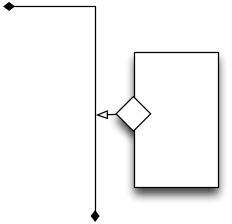
\includegraphics[scale=0.5]{imageSources/sonarturn1.png}
\end{center}
\captionof{figure}{The hovercraft approaching a wall, sonar reading  around 12} 
\label{st1}

As shown in Figure \ref{st1}, as the hovercraft approaches a corner, it will autonomously attempt to stay 12 inches from the wall, thus the sonar will continually read a value close to 12. Both thrust motors will be moving the hovercraft forward at full power.

\begin{center}
 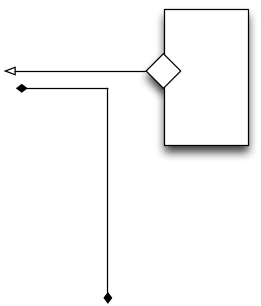
\includegraphics[scale=0.5]{imageSources/sonarturn2.png}
\end{center}
\captionof{figure}{The hovercraft's front half passes  the corner, sonar reading above 60} 
\label{st2}

Figure \ref{st2} shows the hovercraft at a position when the front half of the hovercraft has just passed  the corner, resulting in the sonar reading a value over 60. This implementation assumes the hovercraft is not about to turn down a very short hallway with a dead-end, and so will work for any hallway longer than 60 inches. When the hovercraft enters this state, it turns off the left motor, causing the hovercraft to rotate, and start turning around the corner.

\begin{center}
 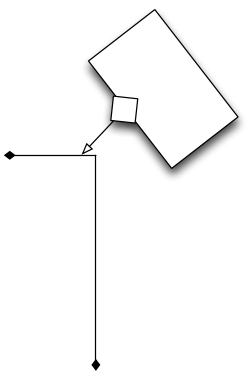
\includegraphics[scale=0.5]{imageSources/sonarturn3.png}
\end{center}
\captionof{figure}{The hovercraft rotates around a corner, resulting in a great decrease in sonar reading value, followed by a sharp increase} 
\label{st3}

As the hovercraft rotates to turn the corner, the sonar readings should decrease greatly. Figure \ref{st3} portrays how the sonar reading will decrease to a minimum value that will be read at the very corner of the wall. Then the readings will begin to start increasing. As the sonar readings begin to increase again, the left motor is signaled to begin thrusting again.

\begin{center}
 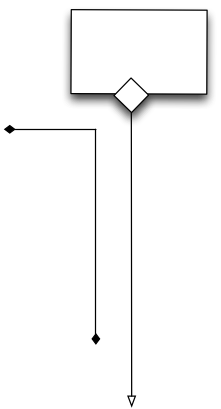
\includegraphics[scale=0.5]{imageSources/sonarturn4.png}
\end{center}
\captionof{figure}{The hovercraft has finished rotating, the sonar again reading above 60} 
\label{st4}

After the hovercraft has rotated almost the full rotation needed to turn the corner, the sonar reading should again read over 60. Figure \ref{st4} shows that when the hovercraft has full turned, and is now facing the desired direction, the sonar points down the hallway the hovercraft had just entered from, and should read a value greater than 60. Both motors should be at full power again, to propel the hovercraft straight down the hallway after successfully rotating around a corner. 
\begin{center}

 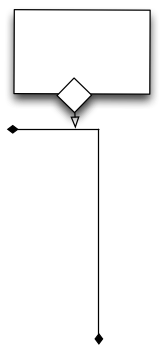
\includegraphics[scale=0.5]{imageSources/sonarturn5.png}
\end{center}
\captionof{figure}{After a successful turn, the hovercraft begins forward movement down the hallway}pdj
\label{st5}

Although all of the rotation necessary to complete a turn was necessary in the first 4 states, Figure \ref{st5} shows the final necessary step in turning around the corner. To steer down a straight hallway, we mentioned above that the sonar controls the hovercraft to stay about 12 inches from the wall. As the hovercraft begins moving forward after finishing the necessary rotation around a corner, it is necessary to switch back to forward controls. When the sonar reads a value under 60 it finishes the turning code and switches back to the code that controls forward movement.
